\chapter{Programmation linéaire}

\section{Définition}

La programmation linéaire est la recherche du maximum ou du minimum d’une fonction (économique le plus souvent) compte tenu de certaines contraintes représentées par des équations ou des inéquations.

\section{Contraintes}

Il existe deux types de contraintes lors de la recherche d’un maximum ou d’un minimum.

\begin{enumerate}
\item Les contraintes d’infériorité du type :  $ax+by\leq c$
sont les limites imposées par l’organisation interne d’une entreprise. On cherche à produire un maximum de marchandises tout en respectant des conditions d’infériorité.
Par exemple, une entreprise souhaite produire le plus possible sachant qu’elle ne peut dépasser les contraintes de productions imposées par la quantité de matière première disponible, le nombre d’ouvriers, les possibilités de stockage, de livraison, etc. 
\item Les contraintes de supériorité du type :  $ax+by\geq c$
sont des limites imposées par l’environnement, par des minima de qualité ou de sécurité. On cherche à acheter ou à produire un minimum tout en respectant des conditions de supériorité.
Par exemple, une entreprise souhaite utiliser le minimum de matières premières tout en respectant les labels de qualité imposés pour la production.
\end{enumerate}

Les variables $x$ et $y$, variables économiques, sont des réels (ou des entiers naturels suivant les cas) toujours positifs. (On ne peut pas produire un nombre négatif d’objets)

\section{Méthode de résolution}

\begin{enumerate}
\item Traduire l’énoncé sous forme de contraintes.
\item Établir un tableau de contraintes.
\item Considérer $x\geq 0$ et $y \geq 0$ (ou autre en fonction des données du problème).
\item Tracer graphiquement les droites intervenant dans les contraintes, puis résoudre graphiquement le système d’inéquations. On obtient le polygone des contraintes (zone du plan vérifiant l’ensemble des contraintes).
\item Trouver graphiquement ou en comparant les pentes le point du plan représentant le maximum ou le minimum. 
\item Tracer graphiquement la fonction représentant le maximum ou le minimum.
\item Calculer les coordonnées  de ce point, puis répondre aux éventuelles questions posées dans le problème.
\end{enumerate}

\begin{exemple}
Une entreprise fabrique deux produits A et B. Le produit A nécessite 2 heures de travail sur la machine M, 3 heures de main-d’œuvre, et 3 kg de matière première. Le produit B nécessite une heure de travail sur la machine M, une heure de main-d’œuvre, et 3 kg de matière première. Le produit A rapporte un bénéfice de Fr. 80.—, le produit B, de Fr. 40.—. Sachant que l’entreprise ne dispose que de 800 heures sur la machine M, 900 heures de main-d’œuvre, et 1500 kg de matière première, déterminer les quantités de produits A et B qu’elle doit fabriquer, afin de réaliser un bénéfice maximum.

\textbf{Tableau des contraintes}

\begin{tabular}{l|l|l|l|}
\cline{2-4}
                                       & Produit A & Produit B & Contraintes \\ \hline
\multicolumn{1}{|l|}{Machine M}        & 2 h       & 1 h       & 800 h       \\ \hline
\multicolumn{1}{|l|}{Main-d'oeuvre}    & 3 h       & 1 h       & 900 h       \\ \hline
\multicolumn{1}{|l|}{Matière première} & 3 kg      & 3 kg      & 1500 kg     \\ \hline
\multicolumn{1}{|l|}{Bénéfice}         & Fr. 80.-- & Fr. 40.-- & maximum     \\ \hline
\end{tabular}

\textbf{Système de contraintes}

$$
\left\{
\begin{array}{lcl}
x&\geq& 0\\
y&\geq & 0\\
2x+y &\leq & 800\\
3x+y &\leq & 900\\
3x+3y &\leq & 1500
\end{array}
\right.
\mbox{ avec } 80x+40y = \mbox{ maximum}
$$

\textbf{Études des droites limites}
\begin{itemize}
	\item $d_1 : 2x+y = 800 \Leftrightarrow y = -2x+800$
			\begin{enumerate}
				\item pente : $-2$
				\item intersection verticale : $x=0 \Rightarrow y = 800$ : $(0;800)$
				\item intersection horizontale : $y=0 \Rightarrow x = 400$ : $(400;0)$
			\end{enumerate}
	\item $d_2 : 3x+y = 900 \Leftrightarrow y = -3x+900$
			\begin{enumerate}
				\item pente : $-3$
				\item intersection verticale : $x=0 \Rightarrow y = 900$ : $(0;900)$
				\item intersection horizontale : $y=0 \Rightarrow x = 300$ : $(300;0)$
			\end{enumerate}
	\item $d_3 : 3x+3y = 900 \Leftrightarrow y = -x+500$
			\begin{enumerate}
				\item pente : $-1$
				\item intersection verticale : $x=0 \Rightarrow y = 500$ : $(0;500)$
				\item intersection horizontale : $y=0 \Rightarrow x = 500$ : $(500;0)$
			\end{enumerate}
	\item $d_M : 80x+40y = M \Leftrightarrow y = -2x+\frac{M}{40}$
			\begin{enumerate}
				\item pente : $-2$
			\end{enumerate}
\end{itemize}

\textbf{Représentation graphique}

\begin{center}
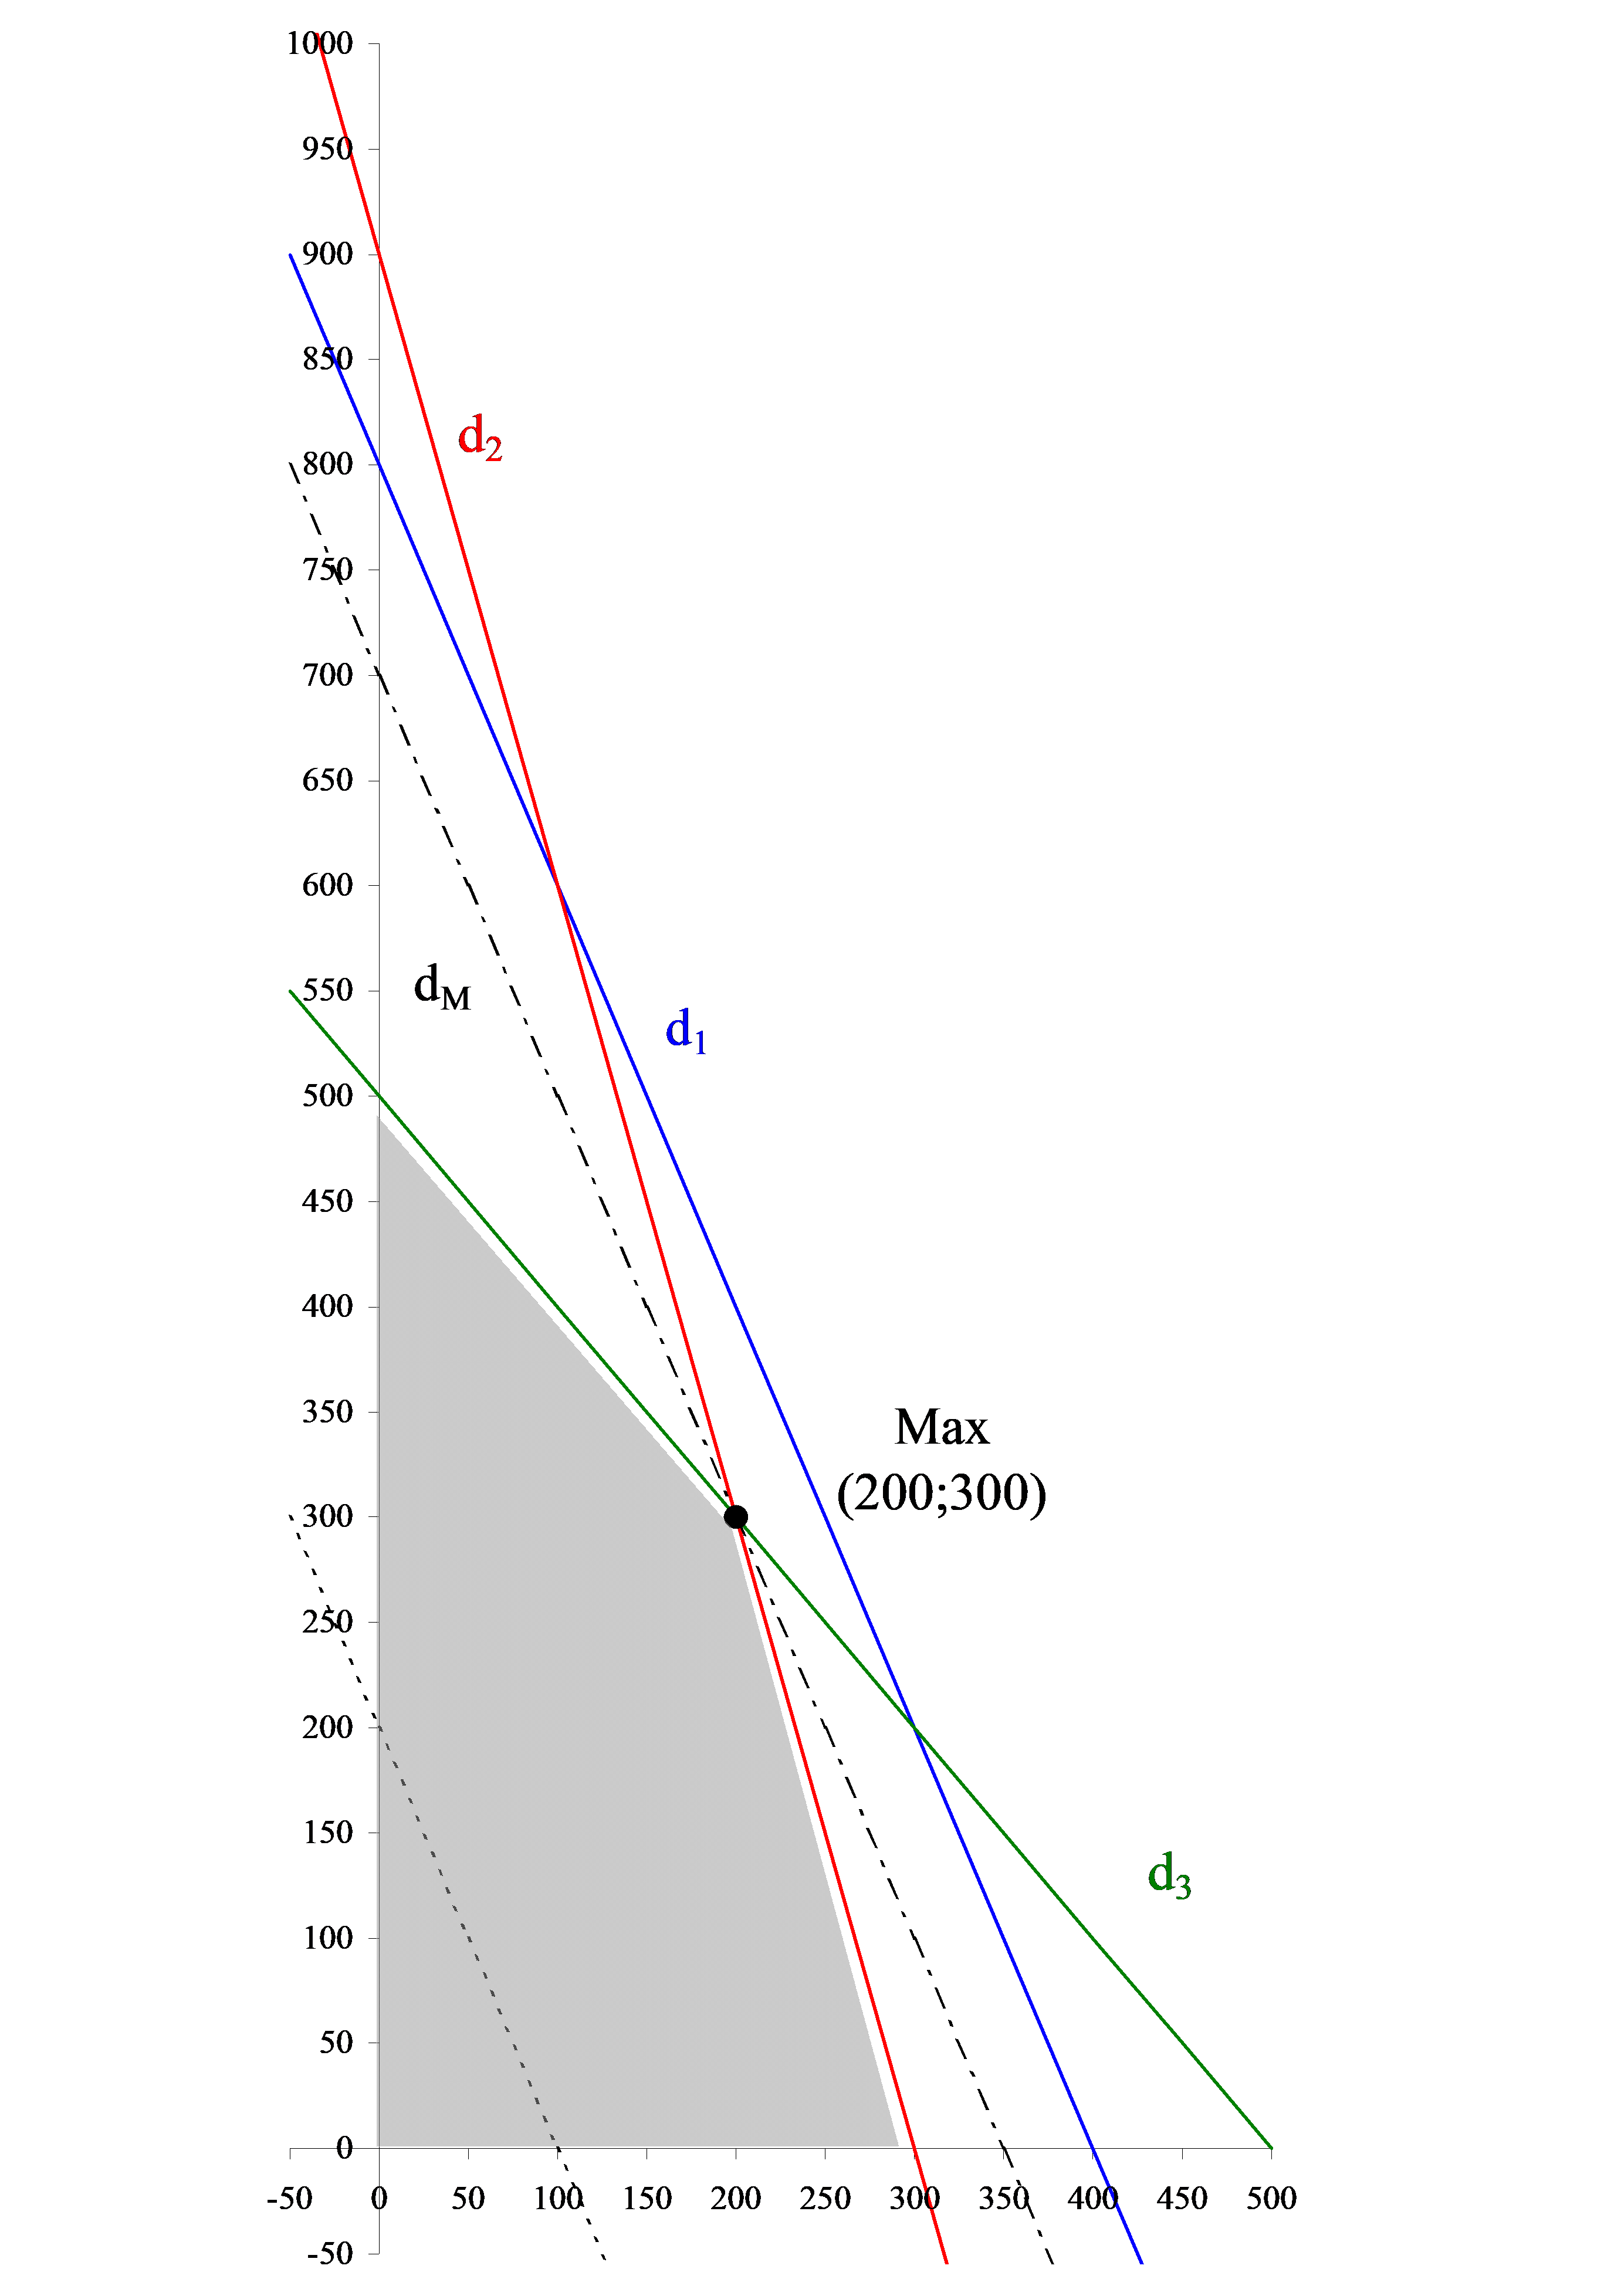
\includegraphics[width = 0.7\textwidth]{programmation/exercice.png}
\end{center}

Le polygone des solutions est donc formé par les axes $x$ et $y$ ainsi que par les droites $d_2$ et $d_3$. On peut ordonner les pentes ainsi :
$$
\begin{array}{|l|l|l|l|}
\hline
x & d_2 & d_3 & y\\
\hline
0 & -1 & -3 & -\infty \\
\hline
\end{array}
$$
La pente de $d_M$ étant de $-2$, la solution se trouve à l'intersection de $d_2$ et $d_3$ car
$$
-1 > -2 > -3.
$$

\textbf{Résolution algébrique}

On résout alors le système $2\times 2$ suivant :
$$
\left\{
\begin{array}{llcl}
d_2 : & 3x+y &=& 900 \\
d_3 : & 3x + 3y &=& 1500
\end{array}
\right.
\Leftrightarrow
\left\{
\begin{array}{lcl}
x &=& 200\\
y &=& 300
\end{array}
\right.
$$

\textbf{Calcul du bénéfice}

On reprend $d_M : 20x + 40y = M$ et on remplace par les valeurs de $x$ et de $y$ trouvées :
$$
80 \cdot 200 + 40  \cdot 300 = 28'000.-
$$

\end{exemple}


\section{Exercices}

\begin{exercice}
Un atelier de confection fabrique deux modèles de robes. L’un exige 3m de tissu et 30h de travail, il procure un bénéfice de Fr. 50.— par robe. L’autre exige 3,5m de tissu et 15h de travail, il procure un bénéfice de Fr. 35.— par robe. 

Sachant que l’atelier dispose de 200m de tissu et de 1200h de travail par jour, quelle quantité de chaque modèle faut-il fabriquer pour que le bénéfice quotidien soit maximum ?

Quel est ce bénéfice ?
\end{exercice}

\begin{exercice}
Une usine fabrique deux types de pièces, P1 et P2. La fabrication nécessite différentes opérations qui seront effectuées sur deux types de machines, M1 et M2. 
Les contraintes de fabrication sont les suivantes :
		
Pour fabriquer une pièce P1, il faut 10 h sur une machine de type M1 , 8 h sur une machine de type M2.
Pour fabriquer une pièce P2, il faut 20 h sur une machine de type M1 , 4 h sur une machine de type M2.

Les machines de type M1 sont disponibles, au total, 4000 h par mois. Les machines de type M2 sont disponibles, au total, 1520 h par mois.
La vente d’une pièce de type P1 rapporte un bénéfice de Fr. 1500.— et la vente d’une pièce de type P2 un bénéfice de Fr. 1000.—.

Quelle est la production mensuelle qui assurera à l’usine un bénéfice maximal ?

Quel sera ce bénéfice ?
\end{exercice}

\begin{exercice}
Dans une cafétéria, on sert deux sortes de desserts glacés, à base de cocktail exotique, de glace et de fruits confits : la coupe créole et la coupe tropicale.
La confection d’une coupe créole nécessite 8 cl de cocktail exotique, 2 dl de glace et 15 g de fruits confits ; celle d’une coupe tropicale 5 cl de cocktail exotique, 2 dl de glace et 25 g de fruits confits.

Sachant que cette cafétéria dispose de 16 litres de cocktail, de 80 litres de glace et de 5 kg de fruits confits et sachant qu’une coupe créole est vendue Fr. 12.— et une coupe tropicale Fr. 10.—, calculer la quantité de chaque coupe à confectionner afin d’obtenir un revenu maximal. 

Quel est ce revenu ?
\end{exercice}

\begin{exercice}
Un artisan fabrique des objets (A) et des objets (B).
La réalisation d’un objet (A) demande Fr. 30.— de matière première et Fr. 125.— de main-d’œuvre celle d’un objet (B) demande Fr. 70.— de matière première et Fr. 75.— de main-d’œuvre.
Pour une bonne gestion de l’entreprise, les dépenses journalières en matière première et en main-d’œuvre ne doivent pas dépasser respectivement Fr. 560.— et Fr. 1250.—. Les profits réalisés sont de Fr. 90.— par objet (A) et de Fr. 45.— par objet (B). 

Déterminer le nombre d’objets (A) et le nombre d’objets (B) que l’entreprise doit produire par jour pour réaliser un profit maximum.

Quel est ce profit ?
\end{exercice}

\begin{exercice}
Il faut pour fleurir un parc au minimum : 1200 jacinthes, 3200 tulipes et 3000 narcisses.
Deux pépiniéristes proposent :
L’un le lot A     : 30 jacinthes, 40 tulipes et 30 narcisses pour Fr. 75.—	
L’autre le lot B : 10 jacinthes, 40 tulipes et 50 narcisses pour Fr. 60.—

Déterminer le nombre de lots A et le nombre de lots B que l’on doit acheter pour que la dépense soit minimale.

Quelle est cette dépense ?
\end{exercice}

\begin{exercice}
Le responsable des manifestations d’une commune a demandé à l’un de ses employés de répondre à la question qui le préoccupe avant Noël.
Il doit orner plusieurs sapins de Noël disséminés sur le territoire communal. Il veut qu’il y ait sur ces sapins au moins 1200 lampes de couleurs variées, 2400 lampes en forme de bougies et 3600 mini-guirlandes. Il a reçu deux offres faites par les deux principaux commerçants de la cité :

\begin{tabular}{|l|l|}
\hline
Première offre               & Deuxième offre               \\ \hline
set préparé avec             & set préparé avec             \\ \hline
6 lampes de couleurs variées & 6 lampes de couleurs variées \\ \hline
18 lampes-bougies            & 6 lampes-bougies             \\ \hline
15 mini-guirlandes           & 30 mini-guirlandes           \\ \hline
Prix du set : Fr. 57.—       & Prix du set : Fr. 75.—       \\ \hline
\end{tabular}

Ce responsable demande à son employé de lui dire :

Comment acheter aux deux commerçants afin de minimiser les dépenses communales pour cet objet ?
Combien dépensera la commune pour l’ornement de ses sapins ?
Combien y aura-t-il de lampes de couleurs variées ?
Combien y aura-t-il de lampes-bougies ?
Combien y aura-t-il de guirlandes ?
\end{exercice}

\begin{exercice}
Une brasserie veut produire deux types de bière ; une bière sans alcool à Fr. 0,50 la bouteille et une bière avec alcool à Fr. 0,40 la bouteille. Pour mettre sur le marché 1000 bouteilles de bière sans alcool, il en coûte à la brasserie

Pour mettre sur le marché 1000 bouteilles de bière sans alcool, il en coûte à la brasserie :

\begin{tabular}{|l|l|}
\hline
Fr. 28.- & De frais de matière première \\ \hline
Fr. 60.- & De frais de brassage         \\ \hline
Fr. 10.- & De frais d'embouteillage     \\ \hline
Fr. 2.-  & De frais de publicité        \\ \hline
\end{tabular}


Pour mettre sur le marché 1000 bouteilles de bière avec alcool, il en coûte à la brasserie :

\begin{tabular}{|l|l|}
\hline
Fr. 20.- & De frais de matière première \\ \hline
Fr. 20.- & De frais de brassage         \\ \hline
Fr. 10.- & De frais d'embouteillage     \\ \hline
Fr. 2.-  & De frais de publicité        \\ \hline
\end{tabular}

Sachant que la brasserie dispose quotidiennement de :

\begin{tabular}{|l|l|}
\hline
Fr. 1'400.- & Pour les frais de matière première \\ \hline
Fr. 2'400.- & Pour les frais de brassage         \\ \hline
Fr. 600.-   & Pour les frais d'embouteillage     \\ \hline
Fr. 300.-   & Pour les frais de publicité        \\ \hline
\end{tabular}

Combien de bouteilles de bière des deux types, la brasserie devra-t-elle produire, pour obtenir un chiffre d’affaires maximum. Calculer le bénéfice réalisé. 
(Graphique : 2 carrés pour 10000 bouteilles). 
En réponse à une nouvelle loi obligeant les brasseurs à mettre sur le marché une bière sans alcool meilleur marché que la bière avec alcool, la brasserie doit modifier ses prix de vente. Elle propose désormais la bière sans alcool à Fr. 0,30 la bouteille et la bière avec alcool à Fr. 0,50 la bouteille. Calculer le nouveau chiffre d’affaires ainsi que le nouveau bénéfice (les frais de production ne varient pas). 
\end{exercice}

\begin{exercice}
Dans une entreprise industrielle de conditionnement de produits alimentaires, un secteur d’activité produit deux barquettes pour la soupe aux légumes :

Barquette “Soupe aux légumes Prodige” pour laquelle l’entreprise utilise :
100 g de choux-fleurs
200 g de carottes
300 g de poireaux

Barquette “Soupe aux légumes Grand-Mère” pour laquelle l’entreprise utilise :
150 g de choux-fleurs
150 g de carottes
400 g de poireaux

Le chef de production a fait, ce jour, un inventaire de ce qu'il possède comme matières premières, soit : 
12 tonnes de choux-fleurs
18 tonnes de carottes
40 tonnes de poireaux

Étant donné l'état de conservation des légumes et afin d'éviter un maximum de pertes sur ces produits, il décide que sa production du jour doit absorber obligatoirement au moins 5 tonnes de choux-fleurs, 15 tonnes de carottes et le $20 \%$ du stock de poireaux. Pour le reste, il désire produire le maximum.

Sachant que sur la barquette “Soupe aux légumes Prodige”, il gagne net Fr. 0.55/pièce et que son gain sur la barquette “Soupe aux légumes Grand-Mère" est de Fr. 0.75/pièce, combien devra-t-il produire de chaque sorte afin de maximiser son bénéfice ?

Quelles quantités de chaque produit de base seront-elles utilisées à la fin de la journée ? 
\end{exercice}

\begin{exercice}
Un pâtissier souhaite proposer à sa clientèle deux assortiments différents de biscuits de Noël.

Pour s’assurer que ses biscuits sont d’une qualité irréprochable, il a indiqué dans les recettes les quantités minimales d’ingrédients que doit contenir chaque assortiment.

\begin{tabular}{lll}
       & Assortiment A & Assortiment B \\
Beurre & 200g          & 100g          \\
Farine & 250g          & 250g          \\
Sucre  & 120g          & 200g          \\
Amande & 30g           & 100g         
\end{tabular}

Le pâtissier doit utiliser pour assurer une production suffisante de biscuits, au minimum 4 kg de beurre, 7,5 kg de farine, 4,8 kg de sucre et 1,5 kg d’amandes. 

Pour proposer suffisamment de choix, le pâtissier désire préparer au minimum cinq assortiments de chaque type.

Sachant que le temps moyen est de 20 minutes pour préparer l'assortiment A et de 40 minutes pour l'assortiment B, calculer :

Combien d'assortiments de chaque type pourra-t-il réaliser en un temps minimum tout en respectant les conditions imposées par les recettes ?

Quelle quantité de beurre, farine, sucre, et amandes va-t-il utiliser ?

Combien de temps faut-il pour préparer l'ensemble des biscuits de Noël ?
\end{exercice}